/*
Congruence Tests
================
This file contains tests for checking the congruence of triangles.
*/

\documentclass[12pt]{article}
\usepackage{amsmath, amssymb}
\usepackage{tikz}
\usepackage{geometry}
\usepackage{titlesec}
\usepackage{graphicx}
\usepackage{float}
\geometry{margin=1in}

\titleformat{\section}{\normalfont\Large\bfseries}{\thesection.}{1em}{}

\title{Congruence of Triangles}
\author{}
\date{}

\begin{document}

\maketitle

\section{Definition}

Two triangles are said to be \textbf{congruent} if they have exactly the same size and shape. This means their corresponding sides are equal in length and their corresponding angles are equal in measure.

\section{Criteria for Congruence of Triangles}

Two triangles are congruent if any one of the following conditions is satisfied:

\begin{itemize}
  \item \textbf{SSS (Side-Side-Side):} All three sides in one triangle are equal to the corresponding three sides in another triangle.
  \item \textbf{SAS (Side-Angle-Side):} Two sides and the included angle of one triangle are equal to the corresponding parts of another triangle.
  \item \textbf{ASA (Angle-Side-Angle):} Two angles and the included side are equal in both triangles.
  \item \textbf{AAS (Angle-Angle-Side):} Two angles and any one side are equal in both triangles.
  \item \textbf{RHS (Right angle-Hypotenuse-Side):} In right-angled triangles, the hypotenuse and one side are equal.
\end{itemize}

\section{Diagrams}

\begin{figure}[H]
\centering
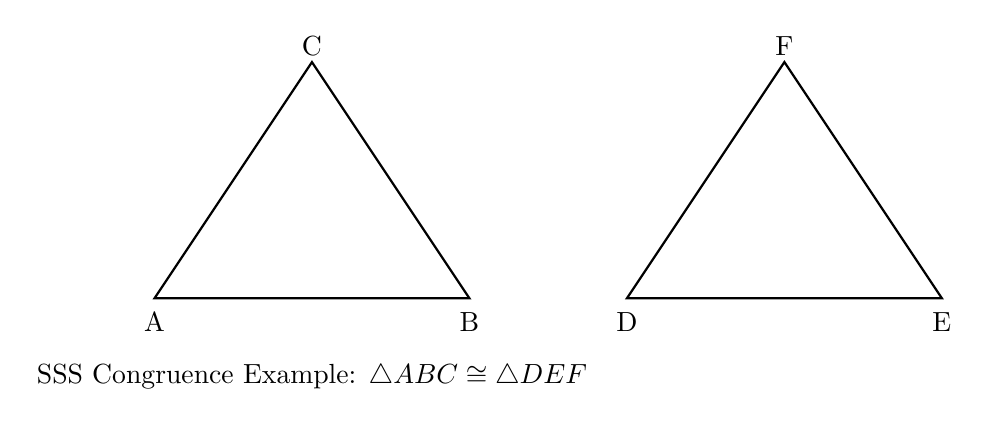
\begin{tikzpicture}[scale=1]
  \draw[thick] (0,0) -- (4,0) -- (2,3) -- cycle;
  \node at (0,-0.3) {A};
  \node at (4,-0.3) {B};
  \node at (2,3.2) {C};

  \draw[thick, shift={(6,0)}] (0,0) -- (4,0) -- (2,3) -- cycle;
  \node at (6, -0.3) {D};
  \node at (10, -0.3) {E};
  \node at (8, 3.2) {F};

  \node at (2, -1.0) {SSS Congruence Example: $\triangle ABC \cong \triangle DEF$};
\end{tikzpicture}
\end{figure}

\section{Example Proof (SSS Criterion)}

\textbf{Given:} In triangles $ABC$ and $DEF$,  
\[
AB = DE,\quad BC = EF,\quad CA = FD
\]

\textbf{To Prove:} $\triangle ABC \cong \triangle DEF$

\textbf{Proof:}

Since all corresponding sides are equal:
\[
AB = DE,\quad BC = EF,\quad CA = FD
\]
By the SSS congruence criterion,  
\[
\triangle ABC \cong \triangle DEF \quad \blacksquare
\]

\end{document}
% End of the document
